\documentclass{article}
\usepackage{amsmath}
\usepackage{titlesec}
\usepackage{graphicx}
\usepackage[margin=1in]{geometry}
\usepackage{hyperref}
\usepackage{amssymb}
\usepackage{subfigure}

% Title, date, and author
\title{Project 3}
\author{Your Name, Collaborator's Name}
\date{\today}

\titleformat{\section}
  {\normalfont\normalsize\bfseries} % Format: font style, size, and weight
  {\thesection}{1em} % Label format and spacing
  {}
  \renewcommand{\thesubsection}{\thesection.\alph{subsection}}

\titleformat{\subsection}
  {\normalfont\small\bfseries} % Format: font style, size, and weight
  {\thesubsection}{1em} % Label format and spacing
  {}
\titleformat{\subsubsection}
  {\normalfont\small\bfseries} % Format: font style, size, and weight
  {\thesubsubsection}{1em} % Label format and spacing
  {}

\begin{document}
\begin{titlepage}
    \centering
    \vspace*{1in}
    
    {\Huge\bfseries Project 2\par}
    \vspace{1.5cm}
    {\Large \today\par}
    \vspace{1.5cm}
    {\Large\itshape Antonio Pampalone 23586519 \\ Giuseppe Pisante 23610012\\ Martina Raffaelli 23616907 \par}
    
    \vfill
    
\includegraphics[width=0.3\textwidth]{FAU-Logo.png}\par\vspace{1cm} % Adjust the width as needed
   
\end{titlepage}

\newpage
\small

\section*{\Large Task 3.0:}
To draw a sketch of the finite-volume discretization domain, it is important to first decide on the type of mesh and variable arrangement. For this task, we opted for a Cartesian mesh, as the domain's geometry is relatively simple and does not require the flexibility of unstructured grids. We chose a staggered arrangement for the variables, where pressure is stored at the center of the control volumes, and the velocity components $u$ and $v$ are located on the faces. This approach helps reduce pressure oscillations and improves the coupling between velocity and pressure, which is particularly beneficial when using the SIMPLE method. Additionally, we adopted a cell-centered storage scheme because it aligns naturally with the flux computation across control volume faces, ensuring consistency and simplicity in the discretization process.
The sketch is reported below:
\begin{figure}[h!]
  \centering
  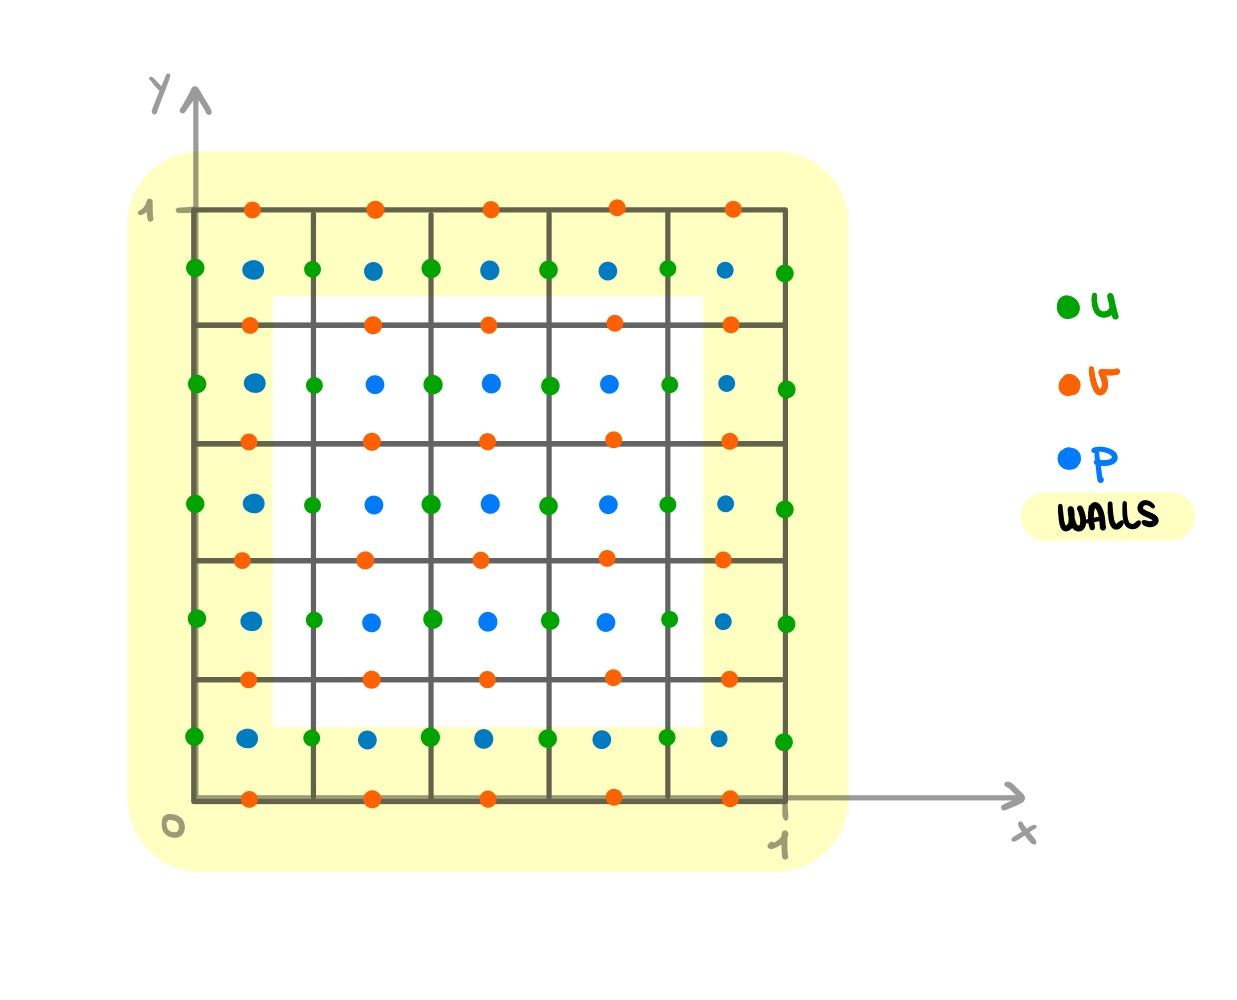
\includegraphics[width=0.5\textwidth]{discretization.jpg}
  \caption{Finite-volume discretization of the domain}
\end{figure}
The yellow line highlights the wall nodes, on which we are going to impose the following boundary conditions:
\begin{itemize}
    \item $v = 0$ on all the walls,
    \item $u = 1$ on the lid,
    \item $u = 0$ on the rest of the walls,
    \item $\frac{\partial p}{\partial n} = 0$ on all the walls.
\end{itemize}
With those boundary conditions we are able to enforce: the motion of the fluid in the proximity of the lid, the no-slip condition on the walls, and the zero-gradient normal condition for the pressure (impermeability of the walls).
In particular we can specify the boundary conditions for the pressure on the single walls as follows:
\begin{itemize}
    \item $\frac{\partial p}{\partial x} = 0$ on right and left walls,
    \item $\frac{\partial p}{\partial y} = 0$ on top and bottom walls.
\end{itemize}


\section*{\Large Task 3.1:}
\section*{\Large Task 3.2:}
\section*{\Large Task 3.3:}
\section*{\Large Task 3.4:}
\section*{\Large Task 3.5:}
\section*{\Large Task 3.6:}
\section*{\Large Task 3.7:}

\begin{thebibliography}{9}
    \bibitem{GitHubRepo}
    \textit{CFD Repository},\\
    Available at: \url{https://github.com/GiuseppePisante/CFD.git}
    
    \bibitem{GitHubCopilot}
    \textit{GitHub Copilot},\\
    GitHub. Available at: \url{https://github.com/features/copilot}
    \end{thebibliography}

\end{document}